\chapter{Implementation}

We have now looked into how systems using procedural content generation can be designed as well as how noise generation works. With this knowledge we can now implement it into unity3D and make our procedural content generator. We will in this chapter look into our project and how we have implemented this. %We will also look into whether or not procedural content generation is a way of saving time while making a game, and there by  answer some of the questions from chapter \ref{ProblemAnalysis}.


\section{Chunk Loader}

As we have talked about in section \ref{WorldGeneration}, it is common for procedural generated world to implement some sort of chunk loader. The chunk loaders job is pretty simple, generate new chunks whenever the player moves towards the end of the world, generate new chunks, so that the player never runs out of area to play on. besides that the chunk loader will remove unused chunks. The chunk loader is there by works as a brain for the world, and decides what to generate.

A code snippet from our chunk loader can be seen in Listing \ref{code:ChunkLoaderStart}. We here see the initial generation of the first $X$ numbers of chunks. The process includes defining the load distance, which is default set to 5 but can be increased, where after the initial load process begins. We hold a reference to all the chunks in a list of lists of gameobjects, which is equivalent to a 2D array. As seen on line 3 we instantiate a new list to hold the reference to the chunks we generate. We then go on to the actual generation of the gameobject, add the components needed, place it at its correct location in the world, and name it so that we can easily look it up if needed. Lastly we add the gameobject to our list and tell the chunk to generate.

\begin{lstlisting}[caption = Code snippet from the start method in the ChunkLoader script., label=code:ChunkLoaderStart, language=Csharp]
for (int i = 0; i < LoadDistance; i++)
{
	List<GameObject> lgo = new List<GameObject>();
	for (int j = 0; j < LoadDistance; j++)
	{
		GameObject go = new GameObject();
		go.AddComponent<Chunk>();
		go.transform.position = new Vector3(((((LoadDistance - 1) / 2) - LoadDistance) + j + 1) * ChunkSize, 0, (((LoadDistance - 1) / 2 - LoadDistance) + i + 1) * ChunkSize);
		go.name = "Chunk" + "[" + (j - Center) + ";" + (i - Center) + "]";
		lgo.Add(go);
		go.GetComponent<Chunk>().Generate();
	}
	Chunks.Add(lgo);
}
\end{lstlisting}

Next we need a way of generating chunk at runtime. In Unity3D we use the "Update" method for this. As seen in Listing \ref{code:ChunkLoaderUpdate}, we depending on the players location, and the center chunk, add now rows or columns, in a similar way as the first initial chunks are generated. We afterwards removes chunks in the opposite end of the world as where we added the new ones. The delete method(s) can be seen in the "ChunkLoader.cs" file in our project, but what is does is it cleans up the terrain(s), removes the references from the list and destroys the gameobject. If we had a world that could be alternated by the player, we should also there save any changes made so that when the player gets back to that chunk the changes made will still be there. But rather than save the whole chunk, only changes made to the chunk should be saved.

\begin{lstlisting}[caption = The Update() method used to generate new chunks., label=code:ChunkLoaderUpdate, language=Csharp]
void Update()
{
	if (Player.transform.position.z < Chunks[Center - 1][Center].transform.position.z + (ChunkSize / 2))
	{
		AddColumnBack();
		DeleteColumnFront();
	}
	if (Player.transform.position.z > Chunks[Center + 1][Center].transform.position.z + (ChunkSize / 2))
	{
		AddColumnFront();
		DeleteColumnBack();
	}
	if (Player.transform.position.x < Chunks[Center][Center - 1].transform.position.x + (ChunkSize / 2))
	{
		AddRowBack();
		DeleteRowFront();
	}
	if (Player.transform.position.x > Chunks[Center][Center + 1].transform.position.x + (ChunkSize / 2))
	{
		AddRowFront();
		DeleteRowBack();
	}
}
\end{lstlisting}

We want to mention that this system is not the most optimal for a chunk loader, which also can be seen when generating new chunks, as the game freezes. A multi threaded event system would have been a better option, however due to Unity3D's poor multi thread support and the time restriction on this project, we decided to lay our focus on other areas. In section \ref{cha:FutureWork} we will discuss this further and how it could be implemented.


\section{World Generator}
\label{WorldGenerator}

With the chunk loader in place we can now move on to implement the chunks them self. As we mentioned in section \ref{WorldGeneration} we only need to generate the world per chunk, and thanks to the coherent noise functionality in libnoise each chunk should have a almost seamless transition. To be extra sure that the chunks are always seamless we do a terrain stitching, meaning we even out the 2 terrains next to each other, with a terrain stitcher. We could skip the stitching step, but this could in some case lead to holes that the player can fall through. Alternatively we could implement our own terrain class, but for this project we will be using Unity3D's built in terrain API, however we will talk about how we could make our own terrain classes in section \ref{cha:FutureWork}.

We will in this section go over some functionality we have created in our chunk generator to mimic terrain in the real world. Some of the functionality may not be used in our final product, but it's there for future development. Additional we will look at a demo that procedurally generates simple island levels, as we wanted to use this as a way to demonstrate and answer if procedural content generation is better, faster and cheaper than having a dedicated level designer to create the levels for games.


\subsection{Island Demo}
\label{IslandDemo}
The island demo scene were made as a baseline comparison to hand made level, as comparing an infinite world to a hand made world could be hard. It took roughly 3 hours to implement the base generation functionality, and roughly an other 3 hours of adding textures, foliage, GUI, regeneration and testing, adding up to a total of 6 work hours on the whole script. We then took this demo scene including the image seen in \figref{fig:IslandDemo} to multiple developing forums and ask for rough time and cost estimate to make a scene like this and we got a few replies that we will talk about in chapter \ref{cha:Conclusion}.

\begin{figure}[H]
	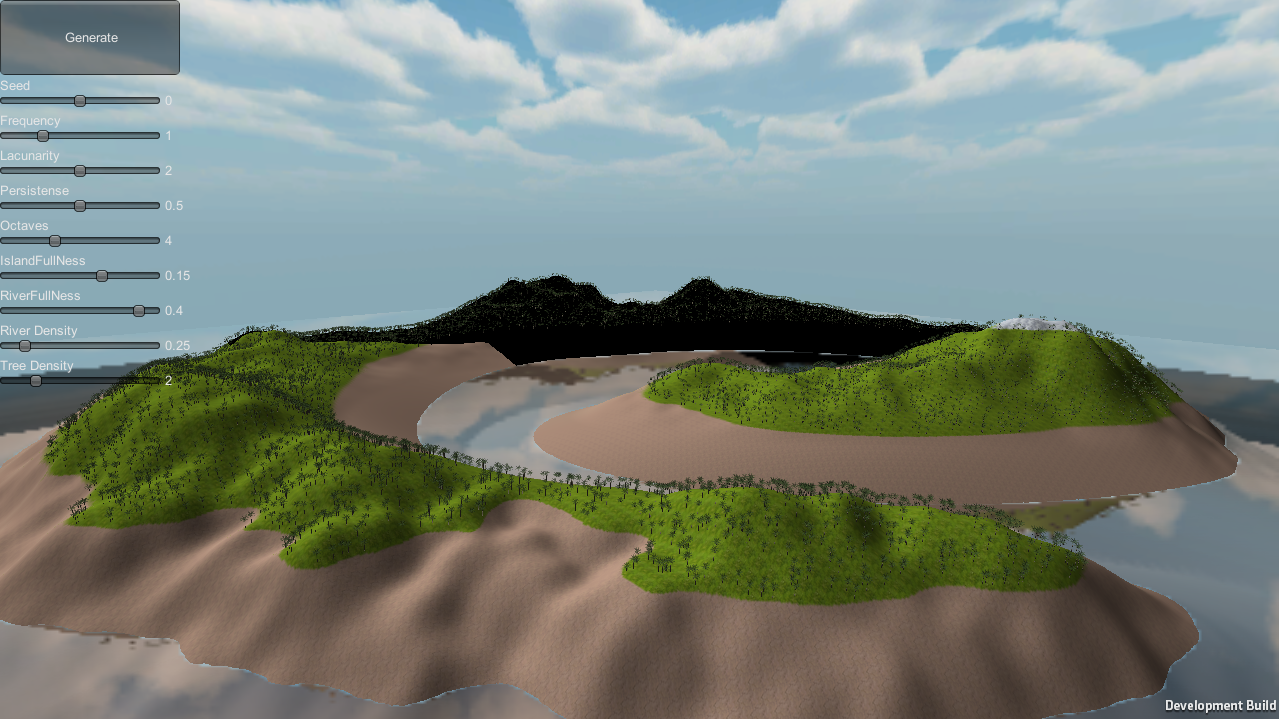
\includegraphics[width=1\linewidth]{img/IslandDemo}
	\centering
	\caption{The first generated island that the user are met with when entering the island demo.}
	\label{fig:IslandDemo}
\end{figure}

Where the island demo we have made for comparison only took a day to create, the other project that we have our main focus have taken us months to make, however as it will have much more details and features put into it, it would seem that the development time needed is increasing exponentially depending on the feature list and extendability of the system. As can see from the island demo, procedural content generators are capable of generating billions of different outputs, simply by changing one or more input values, as can be done at runtime in the island demo. Some result of the generation may be inappropriate for an actual player to play on, but it truly show off the potentials of procedural content generation, and just how fast a simple generator can be made.


\subsection{Biome Map}

To make the world more interesting for the player we have implemented a range of difference biomes. Biomes is like a ecozone, for instance desert, rainforest, tundras to mention a few. We made a biome class where we have base functionality on how the biomes works, and then inherit from there. Each sub class makes is possible for us to define how each biome should be generated and behave. For instance if the world was to generate a tundra we want rough mountainous terrain with very few trees and very little foliage, but a rainforest on the other hand should have many trees and a large a mount of foliage.

The biome map is created from two values, Temperature and humidity. We described in section \ref{NoiseManipulating} how we from combining a gradient mask, which works as a latitude map, with perlin noise create a realistic temperature map that is somewhat similar to how it would be on earth. The humidity map can be a little more tricky to implement and we are there for currently just using a perlin noise map to define humidity. We tried to implement humidity map similar to how it works on earth by using a wind map and create a rain shadow map which we will talk about in section \ref{windmap}, and in section \ref{rainshadowmap}. The reason we took a more simple approach to generating the humidity map was due to the output from the functions generating wind and rain shadow gave us some very weird and unrealistic biome layout and due to the limited time span we decided to focus more on individual biomes.

With the temperature and humidity map in place we can now define our biomes. The way we do this is by implementing a whittaker diagram similar to the one seen in \figref{fig:whittaker}. We can in the whittaker diagram see a biome is depending on temperature and precipitation, also called humidity or rainfall in some context.

\begin{figure}[H]
	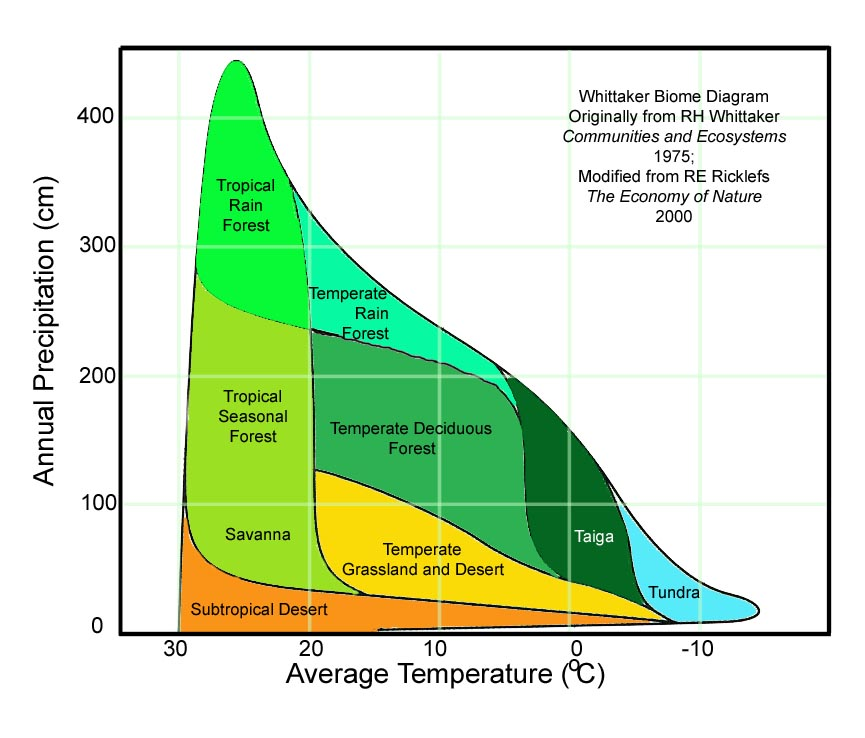
\includegraphics[width=1\linewidth]{img/whittaker}
	\centering
	\caption{The figure shows a whittaker diagram which is used to define ecosystem's temperature and precipitation.}
	\label{fig:whittaker}
\end{figure}

We decide the biome at a point by looping over each value generated by the noise functions as seen in Listing \ref{code:biomedecider}. We then calculate the temperature so that the temperature will be between -50 and 50. We do the same for humidity, but here we change the value depending and the temperature, as we can see from the whittaker diagram that there is very little precipitation/humidity in cold biomes, and do so that the humidity is between 0 and 100. We then at line 9 decide the biome by calling a helper method that returns a enum with the biome type that matches a given temperature and humidity, which is currently defined by if cases to somewhat match the whittaker diagram. Lastly we add the biomes availble in the chunk to a list, this is done so that we later easily can access the biomes for height map generation.

\begin{lstlisting}[caption = A code snippet from the chunk class in our project., label=code:biomedecider, language=Csharp]
for (int i = 0; i < ThisTerain.terrainData.alphamapResolution; i++)
{
	for (int j = 0; j < ThisTerain.terrainData.alphamapResolution; j++)
    {
        Temperature[i, j] = -50.0f + (((((heightMap[i, j] * 0.5f) + 0.5f) + (CosGradient(i + (yOffset * (float)(resolution)), (float)(resolution), 0.25f) * 0.5f) + 0.5f) / 2.0f) * 100.0f);
        
        Humidity[i, j] = ((((CosGradient(i + (yOffset * (float)(resolution)), (float)(resolution), 0.25f) * 0.5f) + 0.5f)) * 100.0f) * (((rainfall[i, j] * 0.5f) + 0.5f));
       
        biomes[i, j] = Biome.DecideBiome(Temperature[i, j], Humidity[i, j]);
        
        if (!availblebiomes.Contains(biomes[i, j]))
        {
        	availblebiomes.Add(biomes[i, j]);
        }	
	}
}
\end{lstlisting}


\subsection{Height Map}

Height mas can be generated in different ways. In our island demo the heightmap is generated first and decide the terrain texture depending on height, however we want biomes to determine the height map and have The height map be dependent on the biomes on a single chunk. For instance we want tundra to be rough mountain terrain, but forest should be much more flat. To do this we use the select module included in libnoise. The select module is a noise manipulation module that takes 2 source modules, and one control module. Depending on the control module's value at a certain point, the select module chooses the values from the 2 source modules, for instance if the control value is -1 the value from the first source module is picked, if the value is 1 it would pick the value from source module 2 and if the value is 0 the two source modules will be blended.

We make a tree structure of select modules as seen in \figref{fig:heightmap} to make a smooth transition between biomes. We have created a biome translator that works as a mask on the biome map, so that a biome of a certain type is mapped as 1. We then smoothen the values so that the mask have a smooth transition between values. The top, left most select module seen in \figref{fig:heightmap} is the module that handles the height map for tundra. We map out the tundra and if the with the biome translator that is used as our control module. If the area is not tundra it takes the value from the second select module that again determines if a certain biome is at a certain point, and this tree can go on until every biomes in a chunk have been mapped, but we have a standard noise in the end so that any biomes that somehow should not have been mapped, have a height map generated with standard values.

\begin{figure}[H]
	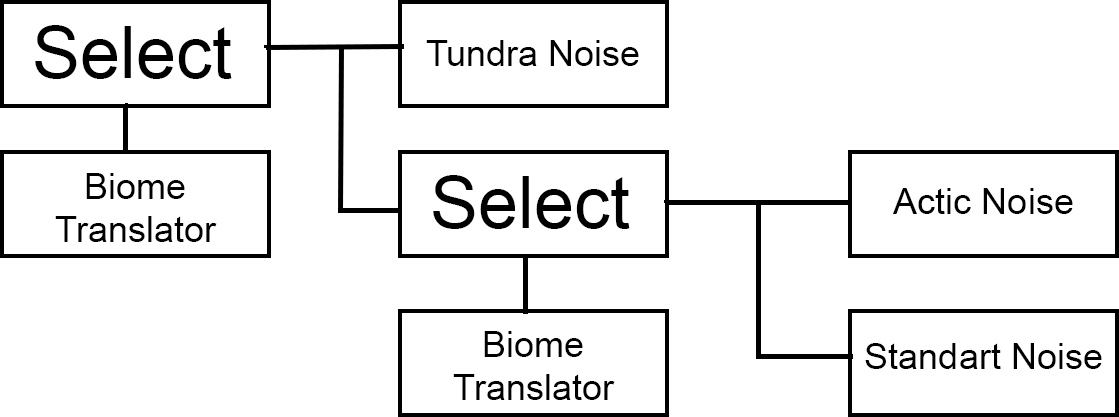
\includegraphics[width=1\linewidth]{img/HeightMap}
	\centering
	\caption{The figure shows a diagram on how a heightmap cointaining 2 biomes is generated.}
	\label{fig:heightmap}
\end{figure}

An alternative way of implementing height maps in a similar way that we tried was to have a single module selecting the values but we ran into some problems with the smoothing of the biome map that would require a larger rewriting of the biome system and generator to fix and it would still work very similar to our current solution. We will try to describe how it could be done in section \ref{cha:FutureWork}.


\subsection{Foliage}

We have defined nature and vegetation objects, such as trees, grass, flowers and so on, as foliage. Foliage is decided by biomes so that each biome have a unique look. Foliage is currently generated by right after the terrain height map and the terrain have been stitched so that we can place the trees at the correct height. When creating a biome we define which tree and how many of each tree should be placed, however we are never sure that all the foliage will actually be placed. The reason for this is due to a biome does not necessarily take up a whole chunk and we take this into account when generating the foliage. In Listing \ref{code:Decorate} we see how we have implemented the foliage decorator. We loop through the decoration array which hold all the game object that should be placed, and then we try to place the specified amount defined. On line 12 we can see the check we do to check whether the location we wanna place the foliage on is of the correct biome type. Since the location is randomized this check is necessary to make sure we don't place foliage in a wrong biome. This way we also indirectly make sure that if a chunk have a specific biome that only take up 10\% of the chunk, a tree have much lower chance to be placed. If we for instance want to place 100 trees but the biome only take up 10\% the chances are that we would have much fewer trees than 100 placed, however according to the law of infinite probability we could at some point have all 100 trees placed, or none trees at all. We then do a raycast to make sure the tree is placed on the ground and doesn't levitate in the air.

\begin{lstlisting}[caption = The decorate function in the Biome class., label=code:Decorate, language=Csharp]
public virtual void Decorate(Chunk chunk)
{
	if (Decorations != null && Decorations.Length > 0)
	{
		for (int i = 0; i < Decorations.Length - 1; i++)
		{
			for (int j = 0; j < Decorationscount[i]; j++)
			{
				int x = DataBaseHandler.DataBase.random.Next(0, DataBaseHandler.ChunkSize);
				int y = DataBaseHandler.DataBase.random.Next(0, DataBaseHandler.ChunkSize);
				
				if (chunk.biomes[Mathf.RoundToInt((((float)DataBaseHandler.BiomeMapSize - (float)1) / (float)DataBaseHandler.ChunkSize) * y), 	Mathf.RoundToInt((((float)DataBaseHandler.BiomeMapSize - (float)1) / (float)DataBaseHandler.ChunkSize) * x)] == Type)
				{
					RaycastHit hit;
					Physics.Raycast(new Vector3(chunk.transform.position.x + x, -1, chunk.transform.position.z + y), Vector3.up, out hit, (float)DataBaseHandler.ChunkSize * 2.5f, 1);
					GameObject go = (GameObject)GameObject.Instantiate(Decorations[i]);
					go.transform.parent = chunk.transform;
					go.transform.localPosition = new Vector3(x, hit.point.y, y);
				}
			}
		}
	}
}
\end{lstlisting}

An alternative way we could generate foliage would be to save all the points containing a specific biome when generating the biomes, and then pick $x$ random point. However this could take up a larger amount of memory depending on how many floating point number we would include. The example in Listing \ref{code:Decorate} is limited to only integers, but by changing the random range to be between 0 and a max value $m$ and then instead placing the gameobject like we do at line 17 we instead would do $DataBaseHandler.ChunkSize * (x / m)$, and the same with $y$.


\subsection{Wind Map}
\label{windmap}

The wind map generator is mainly dependent on the latitude map as the earth's wind directions is dependent on the latitude. We have tried to mimic the way wind directions on earth to create a realistic and earth like world with ideas from Dungeon League\cite{WindMap}. The wind direction map defined by 2D vectors that have been created from a latitude map combined with a perlin noise map, however as dungeon league suggest we could instead of combining the perlin noise and latitude map have distorted the latitude map with a turbulence noise manipulation module. The wind map is currently not used for anything else than generating the rain shadow map that we will talk about in section \ref{rainshadowmap}, however the wind map could have multiple usage in future development. A usage could be for advanced cloud systems, to get the cloud moving in the direction of the wind, or for animating the foliage on the map to make grass and trees bend depending on the wind speed.


\subsection{Rain shadow Map}
\label{rainshadowmap}

Rainsahdows is a nature phenomenon that happens when a place do not receive rain due to the water vapor cools and condenses to form clouds, and make rain fall, when for instance going over a mountain as \figref{fig:Rainshadow} demonstrate.

\begin{figure}[H]
	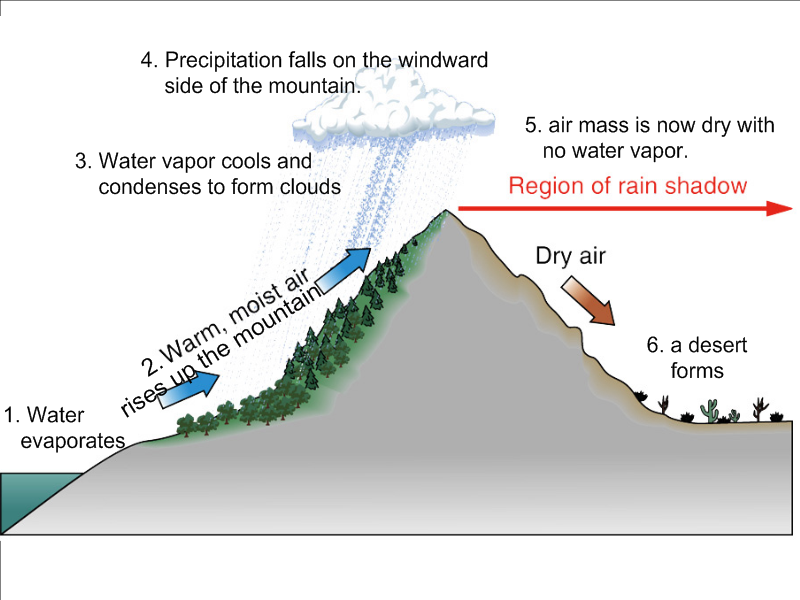
\includegraphics[width=1\linewidth]{img/Rainshadow}
	\centering
	\caption{The figure shows how the rain shadows is created.}
	\label{fig:Rainshadow}
\end{figure}

We have implemented this feature with inspiration from Dungeon League\cite{RainShadowMap}. The idea is to use the wind map we described in section \ref{windmap} and a ray algorithm such a Bresenham's line algorithm\cite{Bresenham}. When ever the height is over a certain threshold at a certain point we shoot a ray in the direction of the wind and the length of a defined wind speed value. We then tried to both displace and combine the rain shadow map with perlin noise, as well as trying to making the line smooth, however we wasn't satisfied with the output and decided not use it in the end, but left it in the source code for possible future development, as both rain shadows and wind add an extra layer of realism to the world.